\documentclass[11pt]{article}

\usepackage[margin=1in]{geometry}
\usepackage{booktabs}
\usepackage{graphicx}
\usepackage{float}
\usepackage{hyperref}
\usepackage{xcolor}
\usepackage{amsmath}
\usepackage{caption}
\usepackage{enumitem}
\usepackage{titlesec}

\hypersetup{colorlinks=true, linkcolor=black, urlcolor=blue, citecolor=black}
\setlist[itemize]{topsep=2pt, itemsep=2pt}
\captionsetup{font=small, skip=6pt}
\titleformat{\section}{\large\bfseries}{\thesection}{0.6em}{}
\titleformat{\subsection}{\normalsize\bfseries}{\thesubsection}{0.6em}{}

\begin{document}

\begin{titlepage}
\hypersetup{pageanchor=false}
\centering
\vspace*{1.2in}
{\LARGE\bfseries Who Wrote It?\\[0.35em]
Identifying LLMs from Their Responses\par}
\vspace{1.1in}
{\large CMPSC 448 Course Project\par}
\vspace{0.8in}
{\large Team leader and sole member\\[0.4em]
\bfseries Shaun Gulati\par}
\vspace{0.6in}
{\large Individual project (not presenting)\\
Default presentation score applies\par}
\vspace{1.2in}
{\large October 11, 2026\par}
\vfill
{\normalsize Department of Computer Science and Engineering\\
The Pennsylvania State University\par}
\end{titlepage}
\hypersetup{pageanchor=true}

\tableofcontents
\newpage

\section{Problem definition}
\label{sec:problem}

Large language models now produce a large share of the text people read. The practical question in this project is whether that text still carries an identifiable author: given a response, can a classifier recover which model wrote it?

The task is four-way classification. Each example is a triple $(\text{model}, \text{instruction}, \text{response})$. The label is the model. The instruction is the user prompt. The response is the model output. The system prompt that UltraFeedback attached to each completion (a randomly sampled ``principle'' such as helpfulness or honesty) is \emph{not} shown to the classifier. Including it would mix a dataset-construction choice into the fingerprint.

Four research questions organize the experiments:

\begin{itemize}
\item \textbf{RQ1.} Using only the response, how accurately can a CNN and an RNN name the model?
\item \textbf{RQ2.} Does the user prompt help? Compare input only, output only, and input concatenated with output. If the prompt alone predicts the model, the dataset rather than the writing style is doing the work.
\item \textbf{RQ3 (extra credit).} Train without one task type and test on that task type. A drop means the classifier was using task-specific habits. A small drop means the fingerprint transfers.
\item \textbf{RQ4 (extra credit).} Measure surface differences (length, lexical diversity, punctuation, markdown) and retrain after those signals are stripped.
\end{itemize}

Chance accuracy and chance macro-F1 are both $0.25$ because the four classes are balanced. Every number below comes from the run recorded in \texttt{results/metrics.json}. The seed is 42.

\section{Dataset curation}
\label{sec:data}

\subsection{Source and license}

The data are the public UltraFeedback release \cite{cui2023ultrafeedback}, hosted as \href{https://huggingface.co/datasets/openbmb/UltraFeedback}{\texttt{openbmb/UltraFeedback}} under the MIT license. UltraFeedback collected about 64k prompts from ShareGPT, UltraChat, Evol-Instruct, TruthfulQA, FalseQA, and FLAN, then asked four models drawn from a pool of roughly seventeen to answer each prompt. This project does not call any model API and does not add private chats.

Upstream prompts have their own histories (ShareGPT conversations, in particular, were written by third parties). The copy used here is the MIT-licensed UltraFeedback redistribution, which is the artifact this repository downloads. Responses shorter than 40 characters, responses that are not strings, and responses that are mostly non-Latin script are removed. Instructions shorter than 12 characters are removed.

\subsection{Models}

The assignment asks for at least three LLM families and a reasonably balanced label set. Four families are used, one checkpoint each:

\begin{center}
\begin{tabular}{lll}
\toprule
Label & Family & Organization \\
\midrule
\texttt{bard} & Bard & Google \\
\texttt{falcon-40b-instruct} & Falcon & Technology Innovation Institute \\
\texttt{gpt-4} & GPT & OpenAI \\
\texttt{llama-2-70b-chat} & Llama & Meta \\
\bottomrule
\end{tabular}
\end{center}

These four were chosen because each comes from a different base-model family and each has thousands of completions on the sources below. WizardLM, Vicuna, and UltraLM were left out on purpose: they are Llama fine-tunes, so a ``family'' label would be muddy. StarChat was left out because it was built for code and would make the code domain a shortcut to the label.

\subsection{A sampling artifact that was removed}

Bard has no completions on \texttt{flan\_v2\_niv2}, \texttt{flan\_v2\_p3}, or \texttt{flan\_v2\_flan2021} (17,939 prompts). Those FLAN items have a very recognizable template (``You will be given a definition of a task\ldots''). If they had been kept, two bad things would follow. Input-only classification could rule out Bard whenever it saw that template. Output-only classification could use the fact that Bard never produced the short FLAN-style answers those templates elicit. Both would be availability artifacts, not fingerprints. Those three sources are excluded. On the sources that remain, all four models were actually queried, and their source counts are similar before balancing.

\subsection{Domain labels}

RQ3 needs a task label. UltraFeedback does not ship one, so each prompt is labeled from the instruction text and the source name. The label does not look at the response. Priority is code, then writing, then reasoning, then question answering. Anything else is dropped (9,681 prompts).

\begin{itemize}
\item \textbf{Code.} A fenced block, a named programming language, or a phrase such as ``write a function'' or ``implement a program.'' The bare word ``function'' is not used; it matches too much ordinary prose.
\item \textbf{Writing.} A request to produce a story, poem, essay, email, article, letter, speech, summary, or similar. Checked after code so ``write a Python script'' stays in code.
\item \textbf{Reasoning.} Whatever remains of \texttt{flan\_v2\_cot}: natural-language inference, multiple choice, and step-by-step word problems, including some arithmetic. This is the mathematics-and-reasoning bucket. A pure ``math'' slice was too small once false positives such as the word ``proof'' in non-math prompts were removed.
\item \textbf{QA.} TruthfulQA, FalseQA, and any remaining prompt that asks a question or begins with what, who, why, how, or explain.
\end{itemize}

The rules are heuristics. A prompt about ``the history of algebra'' can land in QA rather than reasoning, and a ``write a summary'' prompt lands in writing even though it is less open-ended than a short story. The rules are frozen in \texttt{src/domains.py} and were not tuned against classifier accuracy.

\subsection{Balancing and splits}

After filtering, question answering was several times larger than writing. Each model is downsampled, inside each domain, to the same count, and that count is capped at 700. The resulting cell sizes are code 676, QA 700, reasoning 664, and writing 627 per model (10,668 rows, 8,948 distinct prompts). Models are exactly balanced within every domain. Splits are slightly uneven because the split is by prompt, and a prompt may have been answered by only some of the four models.

The released JSONL does not contain the \texttt{id} field shown on the dataset card. The prompt key is the source name plus a SHA-1 prefix of the instruction. All completions of one prompt are assigned to the same split, stratified by domain, at 70/15/15. Overlap of prompt ids between train, validation, and test is zero.

\begin{table}[H]
\centering
\caption{Rows by split and model after balancing.}
\label{tab:splits}
\begin{tabular}{lrrrr}
\toprule
Split & Bard & Falcon-40B & GPT-4 & Llama-2-70B \\
\midrule
Train & 1884 & 1884 & 1877 & 1837 \\
Val & 398 & 374 & 413 & 411 \\
Test & 385 & 409 & 377 & 419 \\
\bottomrule
\end{tabular}
\end{table}

\begin{figure}[H]
\centering
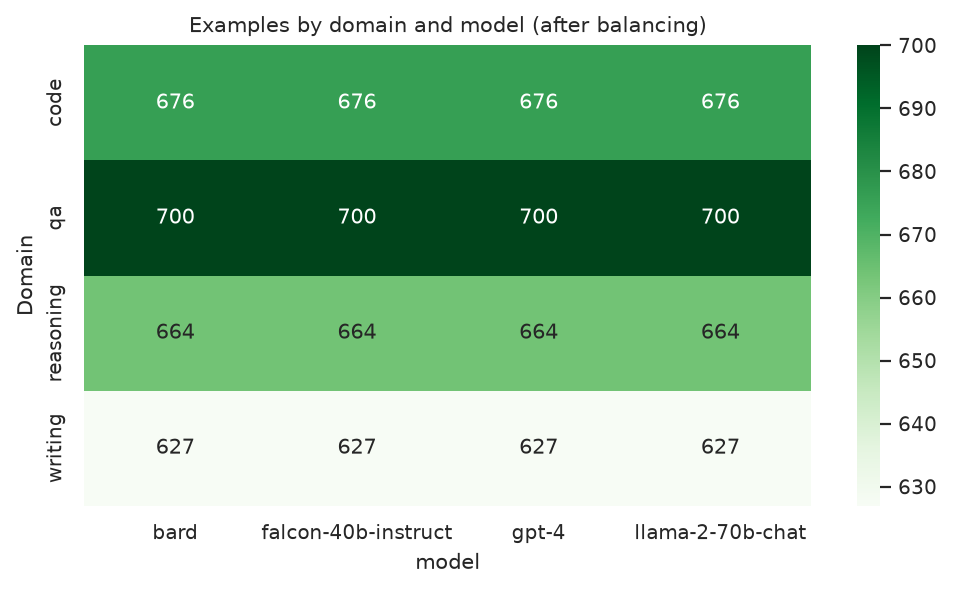
\includegraphics[width=0.72\textwidth]{../results/figures/domain_balance.png}
\caption{Counts by domain and model. Within a domain the four models match.}
\label{fig:balance}
\end{figure}

Responses longer than 6,000 characters are truncated only in the stored text (this affects well under one percent of rows). Length statistics in RQ4 use the word count measured before that cap.

\section{Models and training}
\label{sec:models}

Both required architectures are implemented in PyTorch and trained on CPU. A TF-IDF logistic regression is included as a non-neural baseline so the neural numbers have something to be compared with. It is not a substitute for the CNN or the RNN.

\subsection{Text representation}

Tokens are words and punctuation, lowercased. Case is therefore not available to the networks; punctuation and markdown characters still are, because they are tokens. The vocabulary is the 12,000 most common training tokens with frequency at least 2, plus pad, unknown, and a separator. It is rebuilt for every view and every ablation from that run's training text only. Validation and test tokens that were not seen in training become \texttt{<unk>}.

Sequences are truncated to 128 tokens and padded with zeros. The pad embedding is frozen at zero. For the input+output view, truncation is not applied to the raw concatenation, which would often delete the response. The instruction is limited to 40 tokens, a separator is inserted, and the response is limited to 87 tokens.

\subsection{CNN}

The CNN follows Kim (2014). A 128-dimensional embedding is convolved with filters of width 3, 4, and 5 (96 filters each). Each map is passed through ReLU and collapsed with global max-pooling. The three pooled vectors are concatenated, dropped out with probability 0.5, and mapped to four logits. Max-pooling lets a local phrase, wherever it sits, drive the decision. That is a good match to stock openings (``Sure, here's'') and stock markdown.

\subsection{RNN}

The RNN is a one-layer bidirectional LSTM with hidden size 64 in each direction. Padding is excluded from the recurrence with \texttt{pack\_padded\_sequence}. The final forward and backward states are concatenated, dropped out with probability 0.3, and mapped to four logits. Hidden size 64 is smaller than a typical GPU setup. It is the size that keeps the full RQ1--RQ4 grid on CPU in well under an hour; the CNN is the higher-capacity model in this comparison.

\subsection{Optimization}

\begin{table}[H]
\centering
\caption{Training setup shared by the CNN and the BiLSTM.}
\label{tab:hparams}
\begin{tabular}{ll}
\toprule
Choice & Value \\
\midrule
Loss & Cross-entropy \\
Optimizer & Adam, learning rate $10^{-3}$, weight decay $10^{-5}$ \\
Batch size & 64 \\
Max epochs & 6 \\
Early stopping & Validation macro-F1, patience 2 \\
Checkpoint & Best validation macro-F1, then evaluated once on test \\
Gradient clip & Global norm 1.0 (mainly for the LSTM) \\
Seed & 42 for Python, NumPy, and PyTorch \\
\bottomrule
\end{tabular}
\end{table}

The test set is not used for early stopping or for vocabulary construction. The TF-IDF baseline uses unigrams and bigrams, a minimum document frequency of 2, at most 20,000 features, and logistic regression with $C=2$.

\subsection{What each research question trains}

RQ1 is the output-only CNN and the output-only RNN on the mixed-domain split. RQ2 repeats both architectures on input only and on input+output, plus the TF-IDF baseline on all three views. RQ3 retrains on output text only, once with writing removed from train and validation, and once with code removed. The held-out domain's test prompts are the cross-domain test. The other test prompts are the in-domain comparison for that same model. RQ4 retrains both architectures after each ablation of the response text. Counting the baseline, this is 6 neural runs for RQ1--RQ2, 4 for RQ3, and 8 for ablations.

\section{RQ1: identifying the model from the response}
\label{sec:rq1}

On the mixed-domain test set (1,590 responses), output-only classification is far above the 0.25 chance line. Table~\ref{tab:rq1} gives accuracy and macro-F1. The TF-IDF logistic regression is the strongest of the three. The CNN is close behind it. The BiLSTM is a little lower and, on the validation curve, starts to overfit: its validation macro-F1 peaks at epoch 5 (0.728) and the test numbers use that checkpoint. The CNN's best validation epoch is epoch 6 (0.727), which is also the last epoch allowed, so a longer run might still move the CNN slightly. The cap was fixed before looking at the test set.

\begin{table}[H]
\centering
\caption{RQ1 test performance, output text only.}
\label{tab:rq1}
\begin{tabular}{lcc}
\toprule
Model & Accuracy & Macro-F1 \\
\midrule
CNN & 0.736 & 0.736 \\
BiLSTM & 0.723 & 0.723 \\
TF-IDF + logistic regression & 0.761 & 0.761 \\
\bottomrule
\end{tabular}
\end{table}

\begin{figure}[H]
\centering
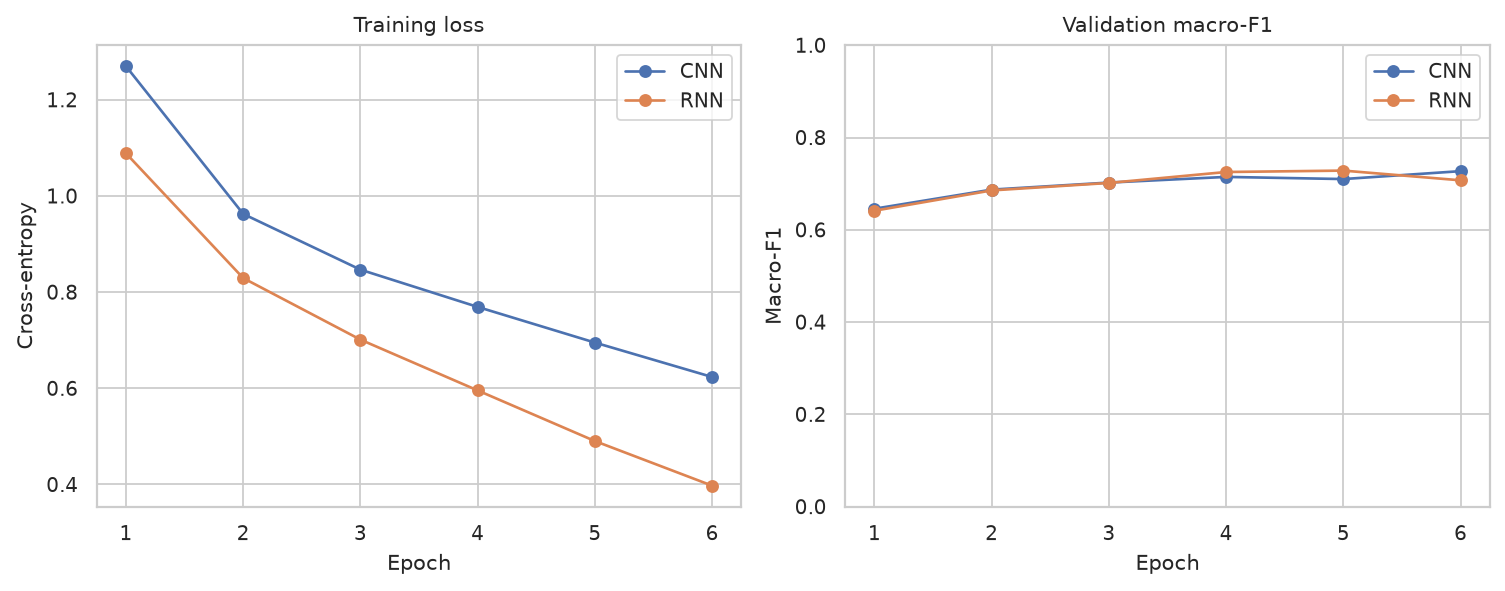
\includegraphics[width=0.92\textwidth]{../results/figures/training_curves_output.png}
\caption{Output-only training. The RNN's training loss keeps falling after validation macro-F1 has flattened.}
\label{fig:curves}
\end{figure}

Per-class scores are in Table~\ref{tab:rq1class}. No class collapses. GPT-4 is the hardest for both neural nets (CNN F1 0.706, RNN F1 0.685). Bard is the easiest for the CNN (F1 0.763, precision 0.825). The TF-IDF model is especially strong on Bard (recall 0.844).

\begin{table}[H]
\centering
\caption{Per-class precision, recall, and F1 on the output-only test set. Supports are 385 (Bard), 409 (Falcon), 377 (GPT-4), and 419 (Llama-2-70B).}
\label{tab:rq1class}
\small
\begin{tabular}{llccc}
\toprule
Classifier & Class & Precision & Recall & F1 \\
\midrule
CNN & Bard & 0.825 & 0.709 & 0.763 \\
CNN & Falcon-40B & 0.764 & 0.719 & 0.741 \\
CNN & GPT-4 & 0.678 & 0.737 & 0.706 \\
CNN & Llama-2-70B & 0.700 & 0.776 & 0.736 \\
\midrule
BiLSTM & Bard & 0.769 & 0.743 & 0.756 \\
BiLSTM & Falcon-40B & 0.697 & 0.741 & 0.718 \\
BiLSTM & GPT-4 & 0.646 & 0.729 & 0.685 \\
BiLSTM & Llama-2-70B & 0.798 & 0.680 & 0.734 \\
\midrule
TF-IDF LR & Bard & 0.772 & 0.844 & 0.806 \\
TF-IDF LR & Falcon-40B & 0.717 & 0.670 & 0.693 \\
TF-IDF LR & GPT-4 & 0.735 & 0.796 & 0.764 \\
TF-IDF LR & Llama-2-70B & 0.821 & 0.742 & 0.779 \\
\bottomrule
\end{tabular}
\end{table}

\begin{figure}[H]
\centering
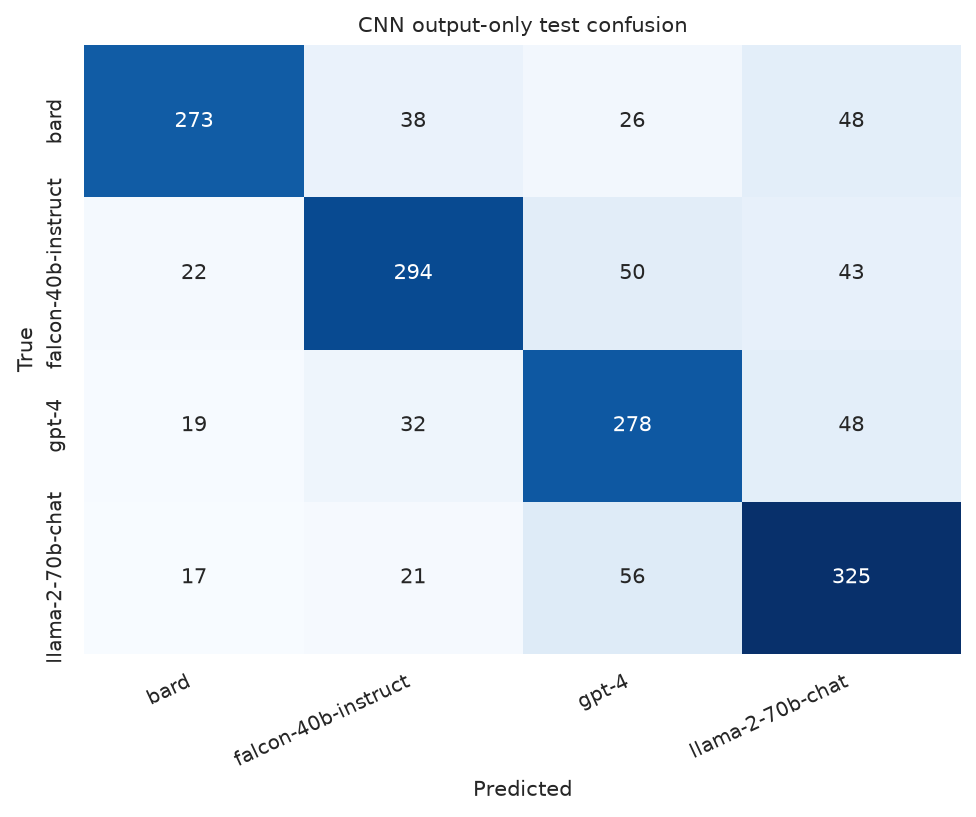
\includegraphics[width=0.46\textwidth]{../results/figures/cm_cnn_output.png}
\hfill
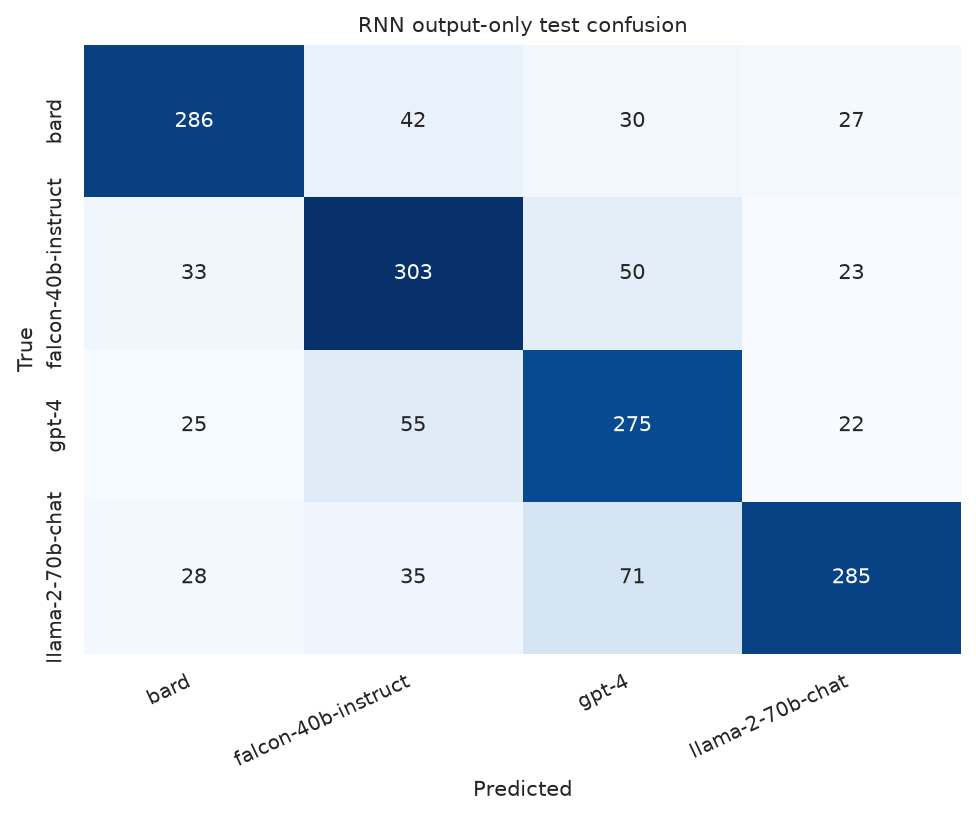
\includegraphics[width=0.46\textwidth]{../results/figures/cm_rnn_output.png}
\caption{Output-only confusion matrices. Rows are the true model.}
\label{fig:cm}
\end{figure}

The largest off-diagonal cells are between GPT-4 and Llama-2-70B. In the CNN, 56 Llama responses are predicted as GPT-4 and 48 GPT-4 responses are predicted as Llama. In the RNN, 71 Llama responses are predicted as GPT-4. Falcon is more often confused with GPT-4 than with Bard (50 CNN errors along that edge). The two long, heavily formatted chat models resemble each other; the errors are not uniform noise.

The same output-only models are uneven across domains even when every domain was seen in training (Table~\ref{tab:bydomain}). Reasoning is easy (CNN macro-F1 0.840). Code, QA, and writing sit near 0.69--0.72. Median response length on reasoning items is 118, 55, 34, and 100 words for Bard, Falcon, GPT-4, and Llama. GPT-4's reasoning answers are much shorter than everyone else's, so part of that domain's accuracy is a length cue. Writing medians are 355, 93, 352, and 334: Falcon is short everywhere, and the other three are long together, which is why writing is harder than the headline accuracy suggests.

\begin{table}[H]
\centering
\caption{Output-only macro-F1 by domain on the mixed-domain test split (the classifier was trained on all four domains).}
\label{tab:bydomain}
\begin{tabular}{lcc}
\toprule
Domain & CNN & BiLSTM \\
\midrule
Code & 0.689 & 0.698 \\
QA & 0.720 & 0.699 \\
Reasoning & 0.840 & 0.800 \\
Writing & 0.690 & 0.683 \\
\bottomrule
\end{tabular}
\end{table}

\section{RQ2: does the prompt help?}
\label{sec:rq2}

It does not. Figure~\ref{fig:rq2} and Table~\ref{tab:rq2} compare the three views. Input-only accuracy is 0.252 for the CNN, 0.273 for the BiLSTM, and 0.260 for TF-IDF. A binomial standard error around chance (0.25) on 1,590 test rows is about 0.011, so the CNN and TF-IDF results sit on the chance line and the RNN's 0.273 is only a small step above it. CNN input macro-F1 (0.218) is below 0.25 because the mistakes are uneven across classes; accuracy is the cleaner summary for this view.

\begin{table}[H]
\centering
\caption{RQ2 test macro-F1 by view. Output-only repeats Table~\ref{tab:rq1}.}
\label{tab:rq2}
\begin{tabular}{lccc}
\toprule
View & CNN & BiLSTM & TF-IDF LR \\
\midrule
Input only & 0.218 & 0.271 & 0.260 \\
Output only & 0.736 & 0.723 & 0.761 \\
Input + output & 0.727 & 0.558 & 0.705 \\
\bottomrule
\end{tabular}
\end{table}

\begin{figure}[H]
\centering
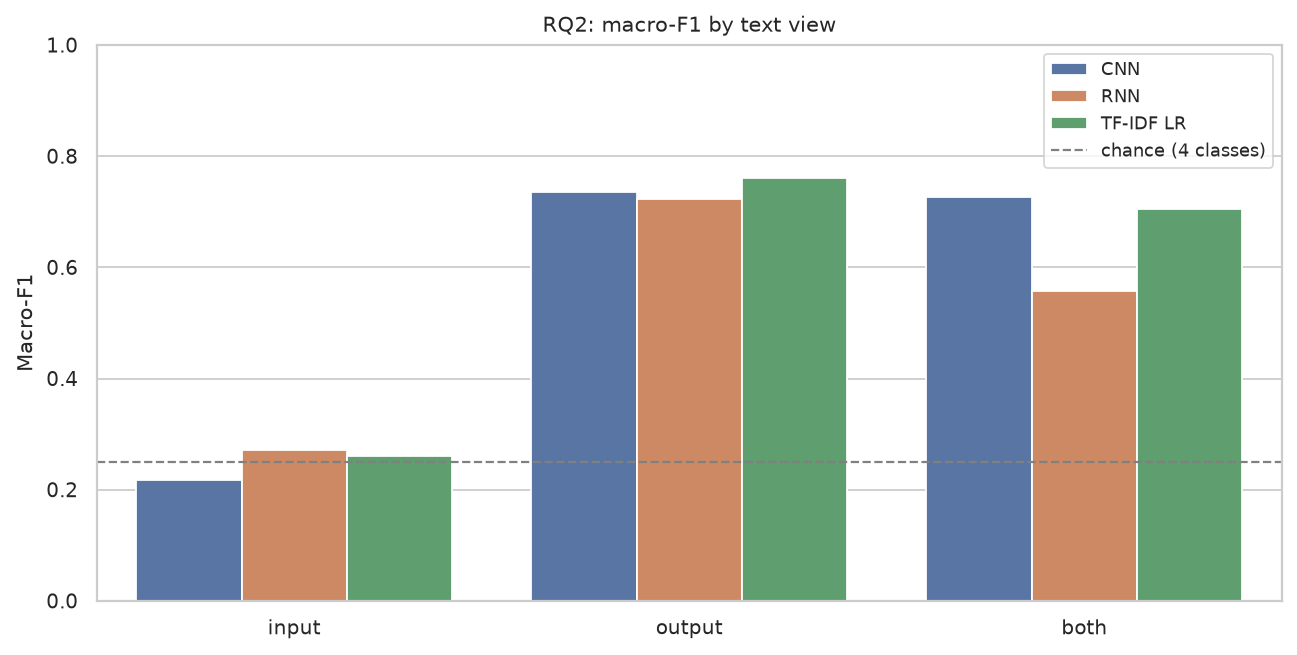
\includegraphics[width=0.88\textwidth]{../results/figures/rq2_views.png}
\caption{Macro-F1 for input only, output only, and both. The dashed line is chance.}
\label{fig:rq2}
\end{figure}

Concatenating the prompt does not improve any model. The CNN drops from 0.736 to 0.727. TF-IDF drops from 0.761 to 0.705. The BiLSTM drops from 0.723 to 0.558. For the bag-of-ngrams model the comparison is the clean one: the prompt adds features and the linear classifier still gets worse, so those features are noise relative to the response. The BiLSTM drop is larger. Two extra facts about that run: the combined view gives the response only 87 tokens, and at epoch 6 the validation macro-F1 is still only 0.563 while training loss is 0.76 (the output-only RNN had already reached a training loss of 0.40). The small LSTM did not finish fitting the longer sequence. I treat the TF-IDF and CNN gaps as the evidence that the prompt does not help, and the RNN gap as that fact plus a capacity limit.

\subsection{Why input-only could have worked, and why it does not here}

The assignment's warning is right in general. If users pick a model, or if a model was online only during some weeks, the prompt distribution becomes a fingerprint of the deployment. I could see a concrete version of that artifact in the raw UltraFeedback files before any training: Bard has zero completions on three FLAN subsets (17,939 prompts) whose instructions use a stock template. Keeping those rows would have let an input-only classifier reject Bard whenever it saw the template, and it would have shifted Bard's output-length distribution because those templates elicit short answers. They were removed before the split.

After that filter, model assignment on the remaining sources is close to random, and each model is forced to the same domain counts. The prompt then carries almost no label information. The small RNN lift (accuracy 0.273) is about what I would expect from a residual mismatch: downsampling is done per model, so the four models do not answer the exact same prompt set. It is not evidence that the user's wording identifies the model.

The practical conclusion is narrow and useful. On this dataset the identifiable signal is in the response. A high input-only score would have meant the split was leaking the label through the prompt, and I would not have trusted the RQ1 number.

\section{RQ3: cross-domain generalization}
\label{sec:rq3}

Two held-out settings were trained from scratch on output text. In the first, train and validation contain code, QA, and reasoning, and the cross test is the writing portion of the original test split (357 rows). The in-domain comparison is the other 1,233 test rows, scored with the same checkpoint. In the second, code is held out (406 cross-domain test rows, 1,184 in-domain). Figure~\ref{fig:rq3} shows the macro-F1 drop.

\begin{table}[H]
\centering
\caption{RQ3 macro-F1. ``In-domain'' is the original test split with the held-out domain removed. The drop is in-domain minus cross-domain.}
\label{tab:rq3}
\begin{tabular}{llccc}
\toprule
Held out & Model & In-domain & Cross-domain & Drop \\
\midrule
Writing & CNN & 0.733 & 0.613 & 0.120 \\
Writing & BiLSTM & 0.714 & 0.637 & 0.077 \\
Code & CNN & 0.749 & 0.644 & 0.105 \\
Code & BiLSTM & 0.716 & 0.667 & 0.049 \\
\bottomrule
\end{tabular}
\end{table}

\begin{figure}[H]
\centering
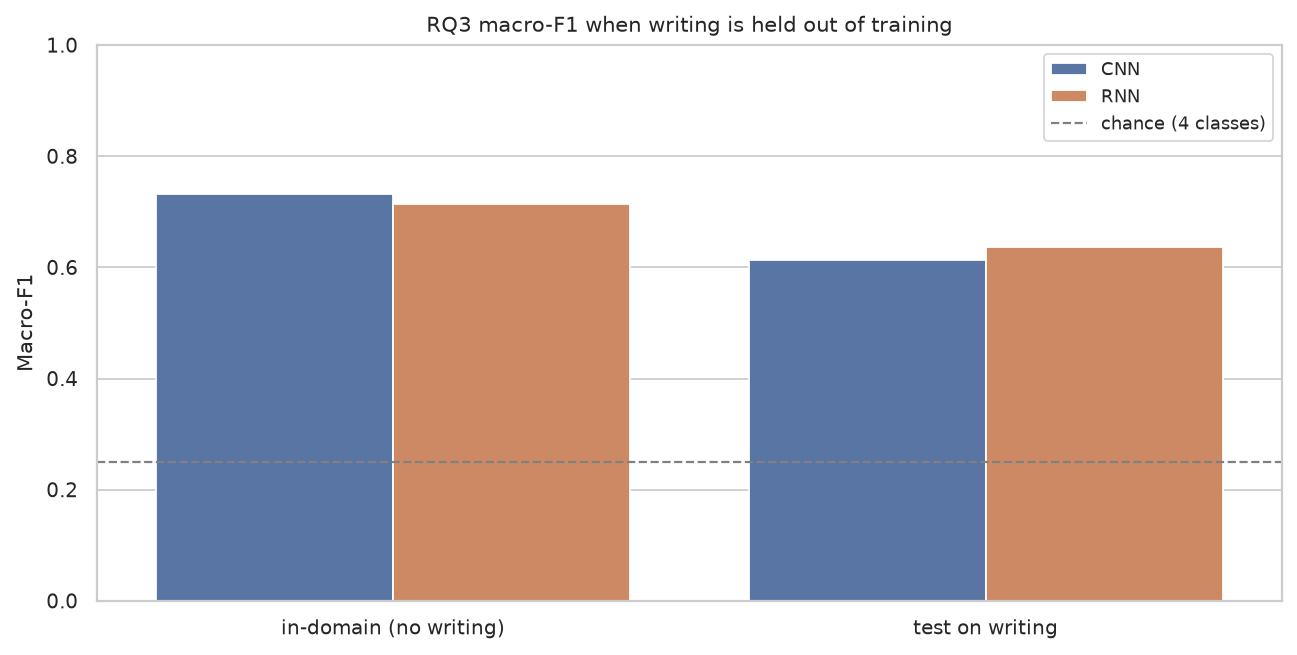
\includegraphics[width=0.48\textwidth]{../results/figures/rq3_writing.png}
\hfill
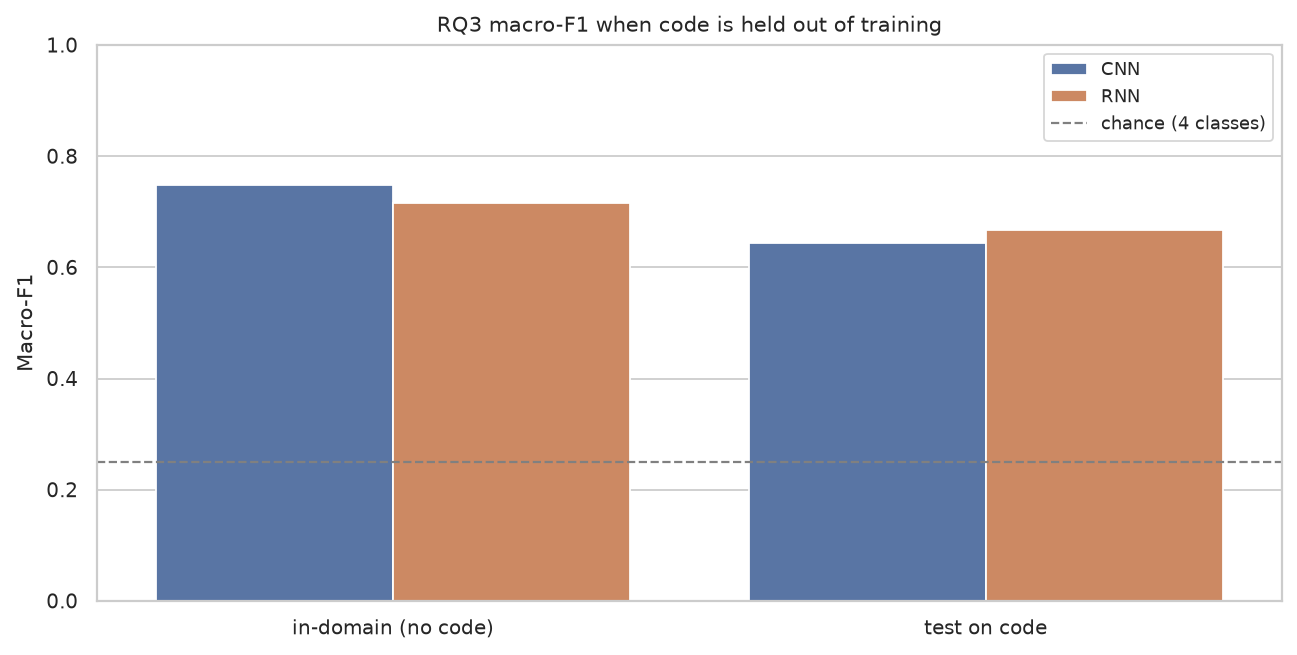
\includegraphics[width=0.48\textwidth]{../results/figures/rq3_code.png}
\caption{Macro-F1 when writing (left) or code (right) is absent from training.}
\label{fig:rq3}
\end{figure}

Performance falls, and it stays well above 0.25. A classifier that had only learned ``this domain's template,'' with no model signal inside the domain, would land near chance on a domain it had never seen. The observed cross-domain macro-F1 (0.61 to 0.67) means a transferable fingerprint exists. The drop (0.05 to 0.12) means some of the in-domain accuracy was task-specific.

Recall by model says the fingerprint is not equally stable (Table~\ref{tab:rq3recall}).

\begin{table}[H]
\centering
\caption{Recall by model, in-domain versus the held-out domain.}
\label{tab:rq3recall}
\small
\begin{tabular}{llcccc}
\toprule
Setting & Model & Bard & Falcon & GPT-4 & Llama \\
\midrule
Writing, CNN in-domain & recall & 0.848 & 0.654 & 0.697 & 0.745 \\
Writing, CNN cross & recall & 0.778 & 0.716 & 0.548 & 0.430 \\
Writing, RNN in-domain & recall & 0.814 & 0.679 & 0.676 & 0.697 \\
Writing, RNN cross & recall & 0.789 & 0.693 & 0.591 & 0.488 \\
\midrule
Code, CNN in-domain & recall & 0.775 & 0.748 & 0.771 & 0.704 \\
Code, CNN cross & recall & 0.531 & 0.660 & 0.716 & 0.648 \\
Code, RNN in-domain & recall & 0.734 & 0.696 & 0.720 & 0.717 \\
Code, RNN cross & recall & 0.625 & 0.641 & 0.706 & 0.686 \\
\bottomrule
\end{tabular}
\end{table}

When the test domain is writing, Llama's CNN recall falls from 0.745 to 0.430 and GPT-4's from 0.697 to 0.548. Bard stays high (0.848 to 0.778) and Falcon does not drop. Llama's writing style is not the style the CNN learned from code, QA, and reasoning. When the test domain is code, the fragile model is Bard: CNN recall falls from 0.775 to 0.531, while GPT-4 barely moves (0.771 to 0.716). Falcon is the most consistent model in both directions. Its responses are short in every domain (median under 100 words; see Section~\ref{sec:rq4}), so the length cue it offers is available whether or not the classifier has seen the task.

I read this as a mixture. Part of the decision is a general habit (how long the answer is, whether it itemizes, which function words it likes). Part of it is a habit that shows up only on some tasks (how Llama writes an essay, how Bard writes code). The cross-domain drop is the second part.

\section{RQ4: which signals are doing the work?}
\label{sec:rq4}

\subsection{Surface measurements}

Figure~\ref{fig:feats} and Table~\ref{tab:feats} describe the responses the classifiers see. Word counts use a letter-word regex on the stored response. Type-token ratio is computed on the first 50 words, and only when the response has at least 50 words (about 17\% of rows are shorter, almost all of them Falcon or reasoning items, and they are omitted from the TTR mean). That fixed window matters: a raw type-token ratio is higher for short texts and would have made Falcon look more ``diverse'' for a purely mechanical reason.

\begin{table}[H]
\centering
\caption{Mean surface statistics by model.}
\label{tab:feats}
\small
\begin{tabular}{lrrrrrr}
\toprule
Statistic & Bard & Falcon & GPT-4 & Llama \\
\midrule
Words (mean) & 260.1 & 117.8 & 230.1 & 268.8 \\
Words (median) & 230 & 76 & 202 & 231 \\
TTR, first 50 words & 0.715 & 0.761 & 0.770 & 0.757 \\
Punctuation per word & 0.190 & 0.170 & 0.231 & 0.200 \\
Code fences & 0.324 & 0.115 & 0.504 & 0.279 \\
Bold markers (\texttt{**}) & 2.31 & 0.07 & 0.30 & 0.09 \\
Bullet lines & 2.85 & 1.07 & 3.08 & 3.00 \\
Markdown hits & 5.77 & 1.37 & 4.08 & 3.56 \\
Exclamation marks & 0.24 & 0.25 & 0.38 & 0.86 \\
Average word length & 4.65 & 4.88 & 5.10 & 4.90 \\
\bottomrule
\end{tabular}
\end{table}

\begin{figure}[H]
\centering
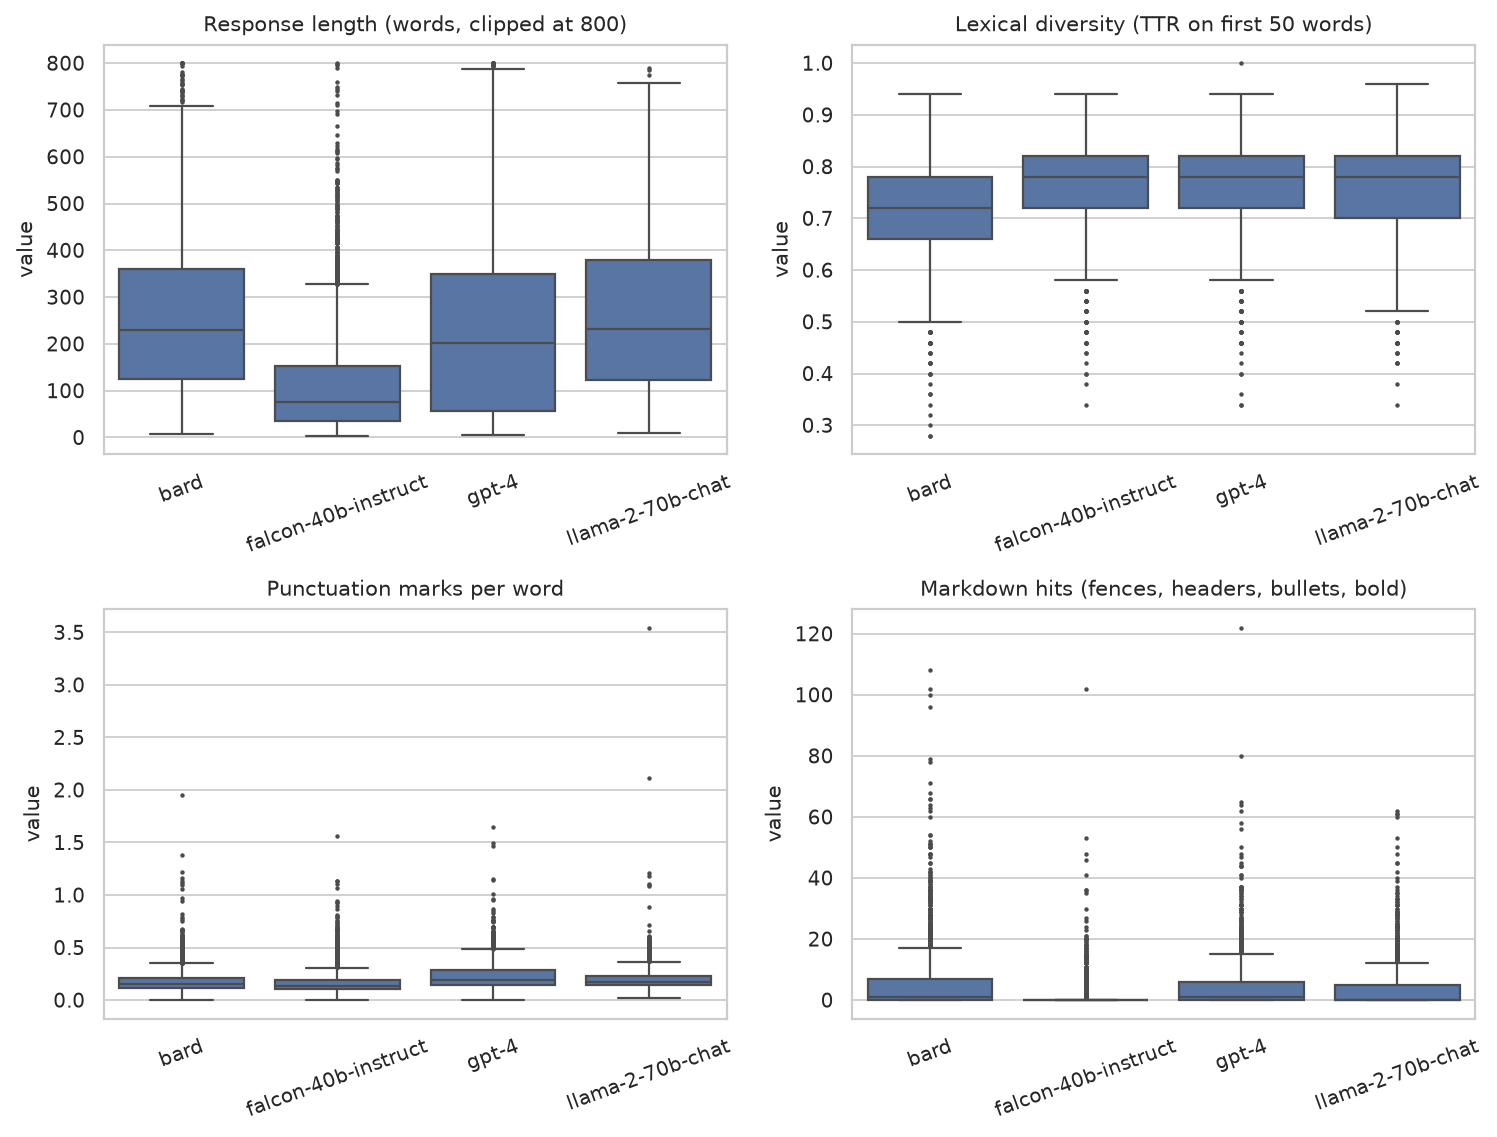
\includegraphics[width=0.95\textwidth]{../results/figures/rq4_features.png}
\caption{Length separates Falcon. Type-token ratio on a fixed 50-word prefix does not. Markdown and punctuation differ in the means; the boxes show that many responses from every model have none.}
\label{fig:feats}
\end{figure}

Four differences are large enough to matter:

\begin{itemize}
\item \textbf{Length.} Falcon's median is 76 words. The other three medians are 202--231. This is the most obvious structural cue, and it is present inside code, QA, reasoning, and writing, not only in the aggregate.
\item \textbf{Markdown.} Bard averages 2.31 bold markers per response; Falcon averages 0.07 and Llama 0.09. GPT-4 averages 0.504 code fences, against 0.115 for Falcon. Bullet lines are common for Bard, GPT-4, and Llama (about 3) and rarer for Falcon (1.07).
\item \textbf{Punctuation.} GPT-4 uses more punctuation per word (0.231) than Falcon (0.170).
\item \textbf{Lexical diversity is not a separator.} Means of the 50-word TTR sit between 0.715 and 0.770. The boxes overlap almost completely.
\end{itemize}

A reader can see the same habits in single examples. One GPT-4 writing answer opens with a formal email header (``Subject: Apology for Delay in Service Delivery''). One Llama answer opens with ``Sure, I'd be happy to help'' and then prints guitar chords. One Bard dialogue is formatted as a screenplay (``INT.\ COFFEE SHOP - DAY''). One Falcon answer to a haiku prompt ignores the form and writes a plain paragraph that names the year 1848 and the materials. Those are individual rows, not the averages, but they match the averages: GPT-4 and Bard spend formatting budget, Llama is long and accommodating, Falcon is shorter and plainer.

\subsection{Ablations}

Each ablation retrains both networks on the transformed response. The test set is transformed the same way.

\begin{itemize}
\item \textbf{Strip markdown.} Fences, inline code, headers, emphasis, and bullet markers are removed. The words inside them stay.
\item \textbf{Fixed length.} Every response is forced to exactly 60 words, by truncation or by repeating the text. Padding length can no longer encode the class.
\item \textbf{Strip punctuation.} Punctuation is deleted and the text is lowercased again (the tokenizer already lowercases).
\item \textbf{All three.} Markdown, then punctuation, then the 60-word constraint.
\end{itemize}

\begin{table}[H]
\centering
\caption{RQ4 ablation macro-F1 on the same test prompts. The drop is measured from that architecture's original output-only score.}
\label{tab:ablate}
\begin{tabular}{lcccc}
\toprule
Condition & CNN & CNN drop & BiLSTM & BiLSTM drop \\
\midrule
Original & 0.736 & --- & 0.723 & --- \\
Strip markdown & 0.738 & $-0.002$ & 0.714 & 0.009 \\
Fixed length (60 words) & 0.713 & 0.023 & 0.684 & 0.039 \\
Strip punctuation & 0.712 & 0.024 & 0.692 & 0.031 \\
All three & 0.684 & 0.052 & 0.656 & 0.067 \\
\bottomrule
\end{tabular}
\end{table}

\begin{figure}[H]
\centering
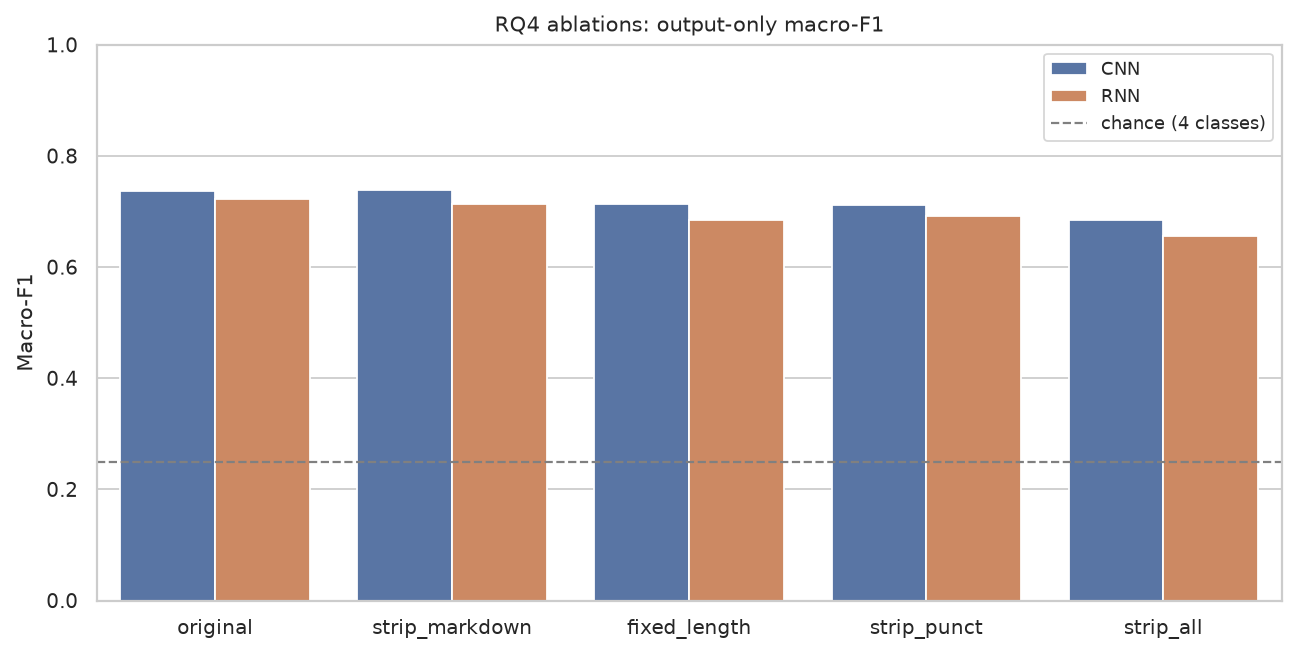
\includegraphics[width=0.88\textwidth]{../results/figures/rq4_ablations.png}
\caption{Output-only macro-F1 after each ablation.}
\label{fig:ablate}
\end{figure}

Stripping markdown does not hurt the CNN (0.738 versus 0.736) and costs the RNN about 0.009. The marker characters were available as tokens, but the words that sat next to them were enough. Forcing a common length costs 0.023 (CNN) and 0.039 (RNN). Removing punctuation costs 0.024 and 0.031. Doing all three costs 0.052 and 0.067. The remaining macro-F1, 0.684 for the CNN and 0.656 for the RNN, is still far above 0.25.

So the classifier is using structural cues, and it is also using lexical ones. Length and punctuation are real, and they are not sufficient to explain the result. After they are gone, word choice still separates the four models. That lines up with TF-IDF beating the neural nets in RQ1: a linear model over word and bigram counts, which only weakly represents order and does not represent raw length except through how many n-grams fire, is already a strong fingerprint detector on this collection.

\section{Lessons and experience}
\label{sec:lessons}

The result I trust most is the pair of negative controls. Output-only macro-F1 is about 0.73. Input-only accuracy is about 0.25 once the Bard/FLAN availability hole is closed. If those two numbers had been similar, I would have been measuring the dataset's sampling scheme. Closing that hole before training, and then watching input-only fall to chance, is what makes the output-only number believable.

The second lesson is that ``an LLM fingerprint'' is too coarse. Falcon is identifiable in part because it is short in every domain, and that cue survives a domain shift. Llama's writing and Bard's code do not match what the classifier learned on the other tasks, and recall for those cells falls hard. A detector that will be applied to a new kind of writing needs the cross-domain number, not the mixed-test number.

The third lesson is about the models I was required to build. On 7,500 training rows, a TF-IDF logistic regression beat both the CNN and the BiLSTM. I do not think that means neural nets cannot represent style. It means that, at this size, with a 12k word vocabulary and a 128-token cap, most of the signal is lexical and a linear model is a better use of the data. The BiLSTM with hidden size 64 was a CPU compromise. Its training loss on the output-only task fell to 0.40 while validation macro-F1 stalled near 0.73, which is overfitting, and on the concatenated view it never caught up. I would rather report that than widen the network after seeing the test score.

Several limits should stay attached to the claims. Domain labels are regular expressions over the prompt, so some ``writing'' rows are summaries and some ``reasoning'' rows are entailment questions rather than mathematics. UltraFeedback wrapped every completion in a random principle prompt (helpfulness, honesty, and so on). The classifier never sees that prompt, but the response was generated under it, which blurs model style with a dataset choice. Sequences are lowercased, so capitalization is invisible to the networks; the uppercase ratio in Table~\ref{tab:feats} is descriptive only. The 60-word ablation repeats short answers until they fill 60 words, which is a blunt way to delete length and could itself create a repetition cue. Test sets for a single domain have a few hundred rows, so a recall difference of a few points is noisy; the Llama writing drop and the Bard code drop are large enough that I do not think they are noise.

What I would do next, with more compute, is keep the same prompt-level split and replace the word CNN with a small pretrained encoder, still frozen or lightly fine-tuned, and check whether the cross-domain drop shrinks. If it shrinks, the missing piece was long-range wording. If it does not, the task-specific habits are real properties of the generators.

\section{Allowed use of LLM tools}
\label{sec:llmuse}

An LLM coding assistant was used to help implement the pipeline, debug training, and draft this report. Every accuracy, F1, confusion count, and feature mean quoted above was produced by running that code and was copied from \texttt{results/metrics.json} or from the feature table computed on \texttt{data/processed/samples.csv.gz}. I am responsible for understanding the dataset, the models, the split, and the claims in this write-up before submitting.

\section{How to reproduce}
\label{sec:repro}

From the repository root, with the packages in \texttt{requirements.txt}:

\begin{verbatim}
python -m src.prepare_data
python -m src.run_all
cd report && pdflatex report.tex
\end{verbatim}

\texttt{prepare\_data} downloads UltraFeedback only if \texttt{data/raw/ultrafeedback/} is empty. The processed file used for the numbers in this report is already in the repository. \texttt{run\_all} retrains every row of Tables~\ref{tab:rq1}--\ref{tab:ablate} at seed 42 on CPU. Early stopping and the epoch cap mean a rerun matches these tables when the library versions match; the committed \texttt{results/metrics.json} is the record of the run this report describes.

\bibliographystyle{plain}
\begin{thebibliography}{1}
\bibitem{cui2023ultrafeedback}
Ganqu Cui, Lifan Yuan, Ning Ding, Guanming Yao, Wei Zhu, Yuan Ni, Guotong Xie, Zhiyuan Liu, and Maosong Sun.
UltraFeedback: Boosting language models with high-quality feedback.
arXiv:2310.01377, 2023.
\bibitem{kim2014cnn}
Yoon Kim.
Convolutional neural networks for sentence classification.
EMNLP, 2014.
\end{thebibliography}

\end{document}
